\documentclass[13pt]{report}

% Ngôn ngữ & font
\usepackage[utf8]{inputenc} % hoặc bỏ nếu compile bằng XeLaTeX/LuaLaTeX
\usepackage[vietnamese]{babel}

% Toán học
\usepackage{amsmath, amssymb, amsfonts}

% Bố cục
\usepackage[left=2.5cm, right=2cm, top=2.5cm, bottom=3cm]{geometry}
\usepackage{setspace}
\usepackage{indentfirst}
\usepackage{enumitem}
\usepackage{fancyhdr}
\usepackage{float}

% Hình ảnh & màu
\usepackage{graphicx}
\usepackage{xcolor}
\usepackage{tikz}
\usepackage{pdfpages}

% Font chữ (chọn 1 trong 2)
% \usepackage{mathptmx} % Times
 \usepackage{mathpazo} % Palatino

% Link & trích dẫn
\usepackage[pdftex]{hyperref}
\usepackage{url}
\usepackage[backend=biber,sorting=none]{biblatex}
\addbibresource{ref.bib}

% Thuật toán & code
\usepackage{algorithm}
\usepackage{algpseudocode}
\usepackage{listingsutf8}

% Code block background
\definecolor{codebg}{rgb}{0.95,0.95,0.95}

\lstdefinestyle{cstyle}{
    language=C,
    backgroundcolor=\color{codebg},
    basicstyle=\ttfamily\small,
    keywordstyle=\color{blue}\bfseries,
    commentstyle=\color{gray}\itshape,
    stringstyle=\color{red},
    % numbers=left,
    % numberstyle=\tiny\color{gray},
    % stepnumber=1,
    % numbersep=10pt,
    frame=single,
    breaklines=true,
    showstringspaces=false,
    tabsize=4,
    captionpos=b
}

\pagestyle{fancy}
\fancyhf{}
\rfoot{\thepage} % Đánh số trang ở chân trang phải
\renewcommand{\headrulewidth}{2pt}
\renewcommand{\footrulewidth}{1pt}

\begin{document}

\thispagestyle{empty}
\fboxsep1em
\fboxrule2pt
\setlength{\baselineskip}{18truept}
\noindent\fbox{
\begin{minipage}
    [c][\dimexpr\textheight-2\fboxsep-2\fboxrule]
    [c]{\dimexpr\linewidth-2\fboxsep-2\fboxrule}
    \begin{center}
				\fontsize{14pt}{20pt}\selectfont 
				{ĐẠI HỌC QUỐC GIA HÀ NỘI}\\
				{TRƯỜNG ĐẠI HỌC CÔNG NGHỆ}\\
				{\bf \textbf{KHOA ĐIỆN TỬ VIỄN THÔNG}} \\
				\vskip 2cm
				\centerline{\includegraphics[height=5cm]{Pictures/logo_UET.png}}
                \vskip 1.5cm
                
                \fontsize{18pt}{20pt}\selectfont 	
				{Báo cáo Thực tập ngành ĐTVT}\\
                \vskip 0.25cm
                \fontsize{18pt}{18pt}\selectfont 
                {\bf \textbf{Công ty Viettel High Tech}}\\
                \fontsize{13pt}{20pt}\selectfont
                
                
                \vskip 3cm
                \fontsize{15pt}{18pt} \selectfont {
                \begin{tabular}{ll}
                    Giảng viên hướng dẫn & \textbf{TS. Nguyễn Hồng Thịnh} \\
                    Sinh viên:  
                    & \textbf{Lê Trần Anh Dũng - 22029041} \\ 
                \end{tabular}{}}

				\vfill
				{\bf Hà Nội - Tháng 9,2025}
			\end{center}
\end{minipage}}


\chapter*{Lời cảm ơn}
\large

Em xin gửi lời cảm ơn chân thành đến cô TS.Nguyễn Hồng Thịnh đã dành thời gian để đọc và góp ý cho báo cáo của em. Những nhận xét và hướng dẫn của cô là nguồn động lực và cũng là cơ sở quan trọng giúp em hoàn thiện hơn trong quá trình nghiên cứu, để các báo cáo được hoàn chỉnh và kỳ thực tập được diễn ra hiệu quả.

Bên cạnh đó, em cũng xin bày tỏ lòng biết ơn sâu sắc đến anh Lê Thanh Bằng - Trưởng phòng Phát triển nền tảng FPGA -
Trung tâm Nghiên cứu thiết bị Vô tuyến băng rộng - Khối 2 - TCT VHT và anh Trung. Trong suốt thời gian thực tập, em đã nhận được sự chỉ dẫn tận tình, những chia sẻ kinh nghiệm quý báu cũng như sự hỗ trợ nhiệt tình từ anh Bằng và anh Trung. Đây là những hành trang vô cùng quan trọng giúp em tiếp cận thực tế công việc, củng cố kiến thức chuyên môn và định hướng rõ ràng hơn cho con đường nghiên cứu, học tập của mình.

Em xin kính chúc cô sức khỏe dồi dào, hạnh phúc và thành công trong công tác giảng dạy và nghiên cứu. Đồng thời, em cũng xin kính chúc anh Bằng và anh Trung luôn mạnh khỏe, nhiều niềm vui và đạt nhiều thành công trong công việc cũng như cuộc sống.

\hspace{8cm} Hà Nội, ngày 23 tháng 8 năm 2025


\newpage
\let\cleardoublepage\clearpage
\large
\tableofcontents
\let\cleardoublepage\clearpage
\newpage
\phantomsection
\listoffigures 
\newpage
\listoftables

\chapter{Mở đầu}
Trong quá trình 6 tuần thực tập tại công ty Vietel High Tech, em đã được giao các đầu việc sau đây:
\begin{figure}[H]
    \centering
    \includegraphics[width=1\linewidth]{Pictures/image.png}
\end{figure}
Tiến độ các tuần: 
\subsubsection{Tuần 1}
Công việc chính: 
\begin{itemize}
    \item Đọc tài liệu tổng quan về 5G: Tìm hiểu các khái niệm như Frame Structure, Numerology, Waveform, Frequency Band, BWP, Synchronization, Beam Management, CSI Framework, Channel Mapping.
    \item Làm quen với FPGA, AI Engine: Tìm kiếm các tài liệu của ADM về AI Engine và chip Versal. 
\end{itemize}
Khó khăn: Chưa có đủ tài liệu hướng dẫn chi tiết về AI Engine, chưa có hiểu biết về các thế hệ mạng trước đó nên khó tiếp cận với kiến trúc 5GNR.
\subsubsection{Tuần 2}
Công việc chính
\begin{itemize}
    \item Tiếp tục nghiên cứu về 5G, kênh PUCCH format 0 ở các lớp L1, L2, L3
    \item Tìm hiểu sâu hơn về AI Eingine trên Versal: kiến trúc của AIE tile, streaming interconnect, DMA, programmable logic, đọc tài liệu từ ADM/Xilinx về sử dụng AIE cho nhân ma trận.
\end{itemize}
Kết quả: Đã hình dung được kiến trúc tổng thể của chip Versal và cách AI Engine hoạt động, các kênh PUCCH hoạt động.
\subsubsection{Tuần 3}
Công việc chính: 
\begin{itemize}
    \item Ghi chép, tổng hợp tài liệu để viết báo cáo về cách tạo chuỗi của kênh PUCCH format 0 và chuẩn bị triển khai kênh này trên MATLAB.
\end{itemize}
Khó khăn: không triển khai được FPGA với AIE do chưa có phần mềm Vitis.

\subsubsection{Tuần 4}
Công việc chính:
\begin{itemize}
    \item Đọc và ghi chép về PUCCH ở lớp vật lý, xử lý bản tin từ UE đến gNB.
    \item Mô phỏng tín hiệu PUCCH format 0 trên MATLAB, thêm nhiễu AWGN (SNR = 10dB).
    \item Phân tích ảnh hưởng của nhiễu đến tín hiệu và chòm sao tín hiệu.
    \item Tìm tài liệu về điều chế và giải điều chế sóng dựa trên chuỗi Zadoff-Chu.
\end{itemize}
\subsubsection{Tuần 5}
Công việc chính:
\begin{itemize}
    \item Xây dựng bộ sinh chuỗi PUCCH format 0 từ các bit HARQ và SR đầu vào.
    \item Mô phỏng toàn bộ quá trình sinh chuỗi trên MATLAB:\begin{itemize}
        \item Tính toán các tham số như $Mzc, Tu,v(n), u, \alpha.$
        \item Sinh chuỗi Zadoff-Chu và áp dụng xoay pha.
        \item Viết lại toàn bộ hàm sinh chuỗi giả ngẫu nhiên theo công thức trong tài liệu.
        \item So sánh kết quả với thư viện MATLAB gốc để kiểm chứng độ chính xác.
    \end{itemize}
\end{itemize}

Kế hoạch tuần tới: Viết hàm decode để trích xuất thông tin HARQ và SR từ tín hiệu nhận được.
\subsubsection{Tuần 6}
Công việc chính:
\begin{itemize}
    \item Xây dựng bộ giải mã chuỗi PUCCH format 0 từ tín hiệu nhận được sau khi được truyền qua kênh nhiễu.
    \item Chỉnh sửa lại code sinh chuỗi trên MATLAB để phù hợp với các điều kiện đầu vào khác nhau.
    \item Báo cáo tổng kết với người hướng dẫn.
\end{itemize}


Trong báo cáo này, em sẽ tập trung vào những khía cạnh tổng quan nhất của 5G và thực thi kênh PUCCH (physical uplink channel) format 0 bằng MATLAB với công đoạn mã hóa và giải mã bằng so sánh tương quan theo tài liệu hướng dẫn của 3GPP và website Sharetechnote. 
Bên cạnh đó, báo cáo này cũng bao gồm những kiến thức cơ bản em tìm hiểu được về kiến trúc của công nghệ AI Engine trên chip Versal theo các tài liệu của nhà sản xuất AMD cung cấp.

Mục tiêu chính của kì thực tập này là củng cố kiến thức nền tảng và tìm hiểu các kiến thức mới về mạng di động 5G, nắm bắt các khái niệm quan trọng trong lớp vật lý của 5GNR, đồng thời rèn luyện kỹ năng triển khai và mô phỏng các kênh vật lý bằng công cụ MATLAB.  

Bên cạnh đó, kì thực tập cũng giúp em bước đầu tiếp cận với công nghệ FPGA và đặc biệt là kiến trúc AI Engine trên chip Versal của AMD, từ đó có định hướng nghiên cứu và ứng dụng cho các đề tài sau này liên quan đến xử lý tín hiệu số tốc độ cao và các hệ thống thông tin không dây.  

Báo cáo được tổ chức thành 3 phần chính:
\begin{itemize}
    \item Phần 1: Tổng quan về 5G new radio.
    \item Phần 2: Thực thi mã hóa và giải mã kênh PUCCH format 0 trên MATLAB.
    \item Phần 3: Kiến trúc AI Engine trên chip Versal. 
\end{itemize}


\newpage
\chapter{Tổng quan về 5G/NR.}
\begin{quote}
    Thời gian nghiên cứu: tuần 1, 2, 3.
\end{quote}

5G/New radio(NR) là thế hệ mạng thứ 5 với tốc độ tối đa được công bố lên tới 20Gbps, so với 1Gbps tối đa của 4GLTE. 5G hứa hẹn sẽ hỗ trợ rất lớn với hệ thông IoT, AI thời gian thực với các xe tự hành, hệ thống thời gian thực....

\section{Kiến trúc.}
\begin{figure}
    \centering
    \includegraphics[width=1\linewidth]{Pictures/kientruc.png}
    \caption{Kiến trúc mức cao.}
    \label{fig:kientruc}
\end{figure}
\begin{itemize}
    \item gNB: trạm gốc 5G, chịu trách nhiệm truyền và nhận sóng tới các thiết bị, bao gồm cả C-plane (Control plane) và U-plane (User-plane).
    \item UE: thiết bị người dùng.
\end{itemize}

Kiến trúc hệ thống của 5G/NR cũng gần tương đương với 4G/LTE được mô tả ở \ref{fig:kientruc}, bao gồm 2 stack đảm nhiệm tùy theo loại dữ liệu được xử lý: C-plane: đảm nhận signaling message trong khi U-plane: đảm nhận dữ liệu người dùng. Cả U-plane và C-plane đều bao gồm những thành phần chung: PHY MAC, RLC và PDCP nhưng các thành phần ơ trên cùng có sự khác nhau. \begin{itemize}
    \item C-Plane: có thêm 2 layer RRC (radio resource control: thành phần điều khiển trung tâm, giúp UE và mạng cấu hình và đồng bộ các lớp giao thức thấp để truyền thông) và NAS (Non-Access Stratum).
    \item U-plane: có thêm 1 lớp SDAP(Service Data Adaptation Protocol để phân loại luồng dữ liệu người dùng) ở trên cùng.
\end{itemize}
\section{Luồng dữ liệu trong hệ thống.}
\begin{figure}[H]
    \centering
    \includegraphics[width=0.8\linewidth]{Pictures/messageflow.png}
    \caption{Luồng dữ liệu trong hệ thống.}
\end{figure}
Quá trình truyền và nhận dữ liệu trong mạng 5G, như minh họa, có thể được mô tả qua các bước sau:
\begin{enumerate}
    \item Người dùng tương tác với ứng dụng trên điện thoại thông minh, tạo ra dữ liệu cần được truyền tải (ví dụ: gửi tin nhắn, truy cập web, xem video).
    \item  Bộ xử lý ứng dụng (Application Processor) và modem trong điện thoại phối hợp để xử lý, mã hóa và đóng gói dữ liệu này theo các giao thức truyền thông phù hợp (bao gồm các tầng như PDCP, RLC, MAC…).
    \item Dữ liệu đã mã hóa được chuyển tới frontend tần số vô tuyến (RF Frontend) của thiết bị, nơi nó được chuyển đổi thành tín hiệu vô tuyến và phát sóng qua ăng-ten.
    \item Trạm gốc (gNB) thuộc mạng truy nhập vô tuyến 5G (5G RAN) sẽ tiếp nhận tín hiệu vô tuyến từ thiết bị người dùng.
    \item Trạm gốc gNB xử lý tín hiệu, sau đó chuyển tiếp dữ liệu tới mạng lõi (Core Network), nơi chịu trách nhiệm điều phối tổng thể mạng và kết nối với Internet.
    \item Mạng lõi định tuyến dữ liệu đến mạng Internet công cộng để đến được máy chủ dữ liệu đích (ví dụ: máy chủ của ứng dụng hoặc website mà người dùng đang truy cập).
    \item Máy chủ dữ liệu tiếp nhận yêu cầu, xử lý và tạo ra phản hồi phù hợp (ví dụ: kết quả tìm kiếm, nội dung video, phản hồi từ ứng dụng…).
    \item Luồng phản hồi đi ngược lại theo trình tự ban đầu: từ máy chủ → qua Internet → đến mạng lõi → đến trạm gốc gNB → phát sóng trở lại đến thiết bị người dùng.
    \item Modem và bộ xử lý ứng dụng trên điện thoại tiếp nhận phản hồi, giải mã và xử lý dữ liệu để hiển thị kết quả cuối cùng cho người dùng thông qua giao diện ứng dụng.
\end{enumerate}
\section{Lớp vật lý}
\begin{figure}[H]
    \centering
    \includegraphics[width=0.6\linewidth]{Pictures/phy.png}
\end{figure}

Lớp vật lý (PHY) trong 5G NR đóng vai trò trung tâm trong việc xử lý tín hiệu vô tuyến, đảm bảo truyền và nhận dữ liệu hiệu quả giữa thiết bị người dùng (UE) và trạm gốc (gNB). Theo hình minh họa, lớp PHY thực hiện các chức năng cốt lõi như đồng bộ thời gian (Time Sync), quét tần số (Frequency Scan), điều khiển công suất (Power Control), báo cáo trạng thái kênh (CSI Report) và phân kênh (Channelization). Ngoài ra, các chức năng như MIMO, quản lý chùm tia (Beam Management) và cấu trúc khung (Frame Structure) thể hiện sự linh hoạt và khác biệt của 5G so với các thế hệ trước, giúp tối ưu hóa hiệu suất truyền dẫn, mở rộng vùng phủ sóng và đáp ứng đa dạng nhu cầu dịch vụ hiện đại.

\subsection{Frame Structure.}
Frame structure đã được thiết kế linh hoạt hơn so với LTE nhằm phục vụ các tác vụ hiện tại như xe tự hành, IoT, truyền video tốc độ cao.
Tài nguyên được chia nhỏ thành các resource block sau đó được chia nhỏ thành các element trên lưới tài nguyên (resource grid). Điều này giúp phân bổ tài nguyên hợp lý tùy theo nhu cầu sử dụng. Bên cạnh đó, khái niệm Numerology là cốt lõi để tạo ra sự linh hoạt này.
\subsubsection{Numerology.}
Một số khái niệm: \begin{itemize}
    \item \textbf{Numerology} (kí hiệu là $\mu$): trong 5G là tập hợp các thông số vật lý định nghĩa cấu trúc sóng mang OFDM 
    \item Subcarrier spacing (SCS): Khoảng cách giữa các sóng con (tính bằng kHz).
    \item Cyclic Prefix (CP): tiền tố vòng để tránh giao thoa đa đường 
    \item Slot length: nhỏ hơn khi subcarrier spacing rộng hơn ($\mu$ nhỏ).
\end{itemize}
Khác với LTE chỉ hỗ trợ một loại subcarrier spacing ở 15kHz, 5GNR hỗ trợ nhiều loại subcarrier spacing tùy theo tham số $\mu$. 
\begin{figure}[H]
    \centering
    \includegraphics[width=0.8\linewidth]{Pictures/numerology.png}
    \caption{Các thông số vật lý trong numerology.\cite{ShareTechnote_5GNR_nume}}
\end{figure}
Với giá trị $\mu$ càng tăng thì khoảng cách giữa các sóng con được nhân đôi theo cấp số nhân 2, thời gian slot giảm, tốc độ truyền nhanh hơn, làm cho băng thông 12 sóng con tăng theo (với $\mu$= 0 thì 12 sub carier là $ 15*12*2^0 = 180$ kHz, với $\mu$ = 6 thì 12 sub carrier là $12* 15* 2^6 = 11520$ kHz).



\textit{Tại sao lại cần nhiều loại subcarrier spacing?}
\begin{itemize}
    \item Subcarrier spacing lớn ($\mu$ cao):
    \begin{itemize}
        \item Symbols ngắn hơn -> truyền nhah hơn.
        \item Phù hợp với tần số cao.
        \item Dùng cho truyền tin siêu nhanh (URLLC), ví dụ: xe tự lái.
    \end{itemize}
    \item Subcarrier spacing lớn ($\mu$ nhỏ):
    \begin{itemize}
        \item Symbol dài hơn -> chống nhiễu tốt hơn.
        \item Phù hợp cho môi trường rộng, nhiều nhiễu.
        \item Dùng cho truyền tải dữ liệu lớn: xem video 4K, tải dữ liệu lớn.
    \end{itemize}
\end{itemize}

\subsubsection{Lưới tài nguyên (Resource Grid).}
Như được mô tả trong hình\ref{regr}, 1 subframe = 1 ms, chứa $14*2^{\mu}$ symbols.
\begin{itemize}
    \item Trục hoành (l): thời gian chia thành các OFDM symbols, gồm $14*2^{\mu}$ được đánh số từ 0 đến $14*2^{\mu} -1$.
    \item Trục tung (k): tần số chia thành các subcarriers.
    \item Resource element(RE): đơn vị nhỏ nhất trong resouce grid, ứng với 1 subcarrier tại 1 OFDM symbol.
    \item Resource block (RB): Ứng với $12N^{RB}_{sc}$ subcarrier liên tiếp trong miền tần số và độ dài tùy chỉnh trong miền thời gian. [38.211-4.4.4.1]
\end{itemize}
\begin{figure}[H]
    \centering
    \includegraphics[width=1\linewidth]{Pictures/resourcegrid.png}
    \caption{Mô tả trực quan của khối dữ liệu trong 1 subframe.\cite{ShareTechnote_5GNR_nume}}

    \label{regr}
\end{figure}
\section{Dạng sóng.}
Khi bắt đầu thiết kế 5G, nhiều waveform mới được đề cập (FBMC, UFMC). Tuy nhiên sau khi đánh giá, OFDM vẫn được sử dụng với tính linh hoạt trong cấu hình. \cite{ShareTechnote_5G_Waveform}
Khái niệm cơ bản về OFDM: 
\begin{itemize}
    \item Các sóng trực giao với nhau, tại thời điểm lấy mẫu của sóng này thì các sóng khác bằng 0.
    \item Nhằm truyền đa kênh.
    \item Tuy nhiên trong không gian cũng có nhiễu làm trôi tần số, gây ra ảnh hưởng của các kênh lên nhau.
    \item Cách xử lý: thêm cyclic prefix và để xử lý lỗi chồng lấn.
\end{itemize}

\chapter{Sinh và phát hiện chuỗi dựa trên tương quan để giải mã UCI trong PUCCH format 0.}
\begin{quote}
    Thời gian nghiên cứu: tuần 3, 4, 5, 6.
\end{quote}
\section{Khái quát về kênh PUCCH và các format.}
 Kênh PUCCH (Physical Uplink Control Channel) là kênh vật lý đường lên trong hệ thống 4G LTE và 5G NR, được thiết kế để truyền các thông tin điều khiển ngắn gọn (\textbf{UCI}) từ thiết bị đầu cuối (UE) về trạm gốc (gNB/eNB). Thông tin này thường bao gồm các chỉ số phản hồi (Hybrid Automatic Repeat Request Acknowledgment - \textbf{HARQ-ACK}), báo hiệu yêu cầu tài nguyên đường lên (Scheduling Request - \textbf{SR}) và các giá trị chỉ thị chất lượng kênh (Channel State Information - \textbf{CSI}).\cite{kivijakola2024pucch}
 
 Khác với kênh PUSCH, vốn mang dữ liệu người dùng, PUCCH chỉ tập trung vào dữ liệu điều khiển nhằm đảm bảo kết nối hiệu quả và duy trì liên lạc ổn định. Tùy theo dung lượng thông tin và yêu cầu độ tin cậy, PUCCH được chuẩn hóa thành nhiều định dạng khác nhau, trong đó mỗi định dạng có cơ chế ánh xạ tài nguyên và phương pháp điều chế riêng.

 Có 5 format để lựa chọn (0, 1, 2, 3, 4) tùy vào các đặc điểm:
    \begin{itemize}
        \item 0, 1 dùng để mang số lượng  UCI bit <= 2. 
        \item 0, 2 là short PUCCH vì nó chỉ dài 1-2 symbols.
        \item 1, 3, 4 là long PUCCH vì dài 4 -> 14 symbols.
        \item 0, 1, 2 được sử dụng nhiều hơn.
\end{itemize}
Báo cáo này tập trung nghiên cứu kênh PUCCH Format 0, với trọng tâm là các công thức mã hóa (encode) và giải mã (decode) tín hiệu.  
    
    Format 0:
    \begin{itemize}
        \item Loại: short PUCCH.
        \item Độ dài: 1-2 OFDM symbols.
        \item UE multiplexing: có, tối đa 12 UE.
        \item Dạng tín hiệu: dựa trên Zadoff-Chu sequence và cyclic shift.
    \end{itemize}

\section{Công thức liên quan.}


\subsection{Tính tương quan.}
Tương quan giữa hai chuỗi tín hiệu là một phép đo mức độ giống nhau giữa chúng khi một chuỗi được dịch chuyển tương đối so với chuỗi còn lại. Trong xử lý tín hiệu, tương quan thường được sử dụng để phát hiện mẫu, trích xuất đặc trưng hoặc đo độ trễ giữa các tín hiệu.

Cho hai chuỗi tín hiệu rời rạc \( x[n] \) và \( y[n] \), hàm tương quan chéo (cross-correlation) được định nghĩa như sau:

\begin{equation}
R_{xy}[k] = \sum_{n = -\infty}^{\infty} x[n] \cdot y[n + k]
\end{equation}

Trong thực tế, với tín hiệu hữu hạn chiều dài \( N \), công thức được viết lại như sau:

\begin{equation}
R_{xy}[k] = \sum_{n = 0}^{N-1} x[n] \cdot y[n + k]
\end{equation}

Khi \( x[n] = y[n] \), ta thu được hàm tương quan tự thân (auto-correlation):

\begin{equation}
R_{xx}[k] = \sum_{n = 0}^{N-1} x[n] \cdot x[n + k]
\end{equation}

Giá trị \( R_{xy}[k] \) đạt cực đại khi hai chuỗi giống nhau nhất tại độ dịch \( k \), từ đó có thể xác định độ trễ hoặc mức độ đồng bộ giữa hai tín hiệu.

\section{Công thức điều chế kênh PUCCH format 0.}

\subsection{Chuỗi Low-PAPR (Low peak-to-average-power ratio).}
 Format 0 sử dụng phương trình chuỗi LPAPR loại 1, và cấu trúc của nó được minh họa trong Hình 14. Phương trình: 
\[
r^{\alpha ,\delta }_{u,v}(n) = e ^{j\alpha n}\overline{\rm r}_{u,v}(n),   \space 0 \leq n < M_{ZC}
\]
 
 Chuỗi bao gồm hai thành phần: phần quay pha $e^{j\alpha n}$ và phần chuỗi gốc $\overline{\rm r}_{u,v}(n)$. Phần chuỗi gốc là chuỗi Zadoff-Chu. Thành phần quay pha được sử dụng để ghép kênh nhiều UE cùng chia sẻ các tài nguyên vật lý giống nhau và mang dữ liệu UCI trong trường hợp format 0. 
 
\begin{figure}[H]
    \centering
    \includegraphics[width=1\linewidth]{Pictures/processing chain.png}
    \caption{Quá trình tạo chuỗi Low-PAPR.\cite{kivijakola2024pucch}}
    \label{fig:enter-label}
\end{figure}


\subsection{Độ dài chuỗi ZC: M\textsubscript{ZC}}
Được tính theo \[ M_{ZC} = mN^{RB}_{sc}/2^{\delta} \] với các giá trị:
\begin{itemize}
    \item $m$ là số RB được sử dụng, ở đây format 0 thì $m=1$.
    \item $N^{RB}_{sc}$: số subcarrier trên 1 resource block, ở đây là 12 (chiều rộng tần số là 12).
    \item $\delta =0$. 
\end{itemize}
 Bằng việc có được độ dài chuỗi, ta tìm chuỗi ZC.
\subsection{Chuỗi cơ sở $\overline{\rm r}_{u,v}(n)$}
\[
\overline{\rm r}_{u,v}(n)=e^{j\phi(n)\pi/4},\space  0 \leq n \leq M_{ZC}-1 \label{pt r}
\]
 Với việc đối chiếu giá trị \textbf{$u$} với bảng giá trị đã được tính toán trước của chuỗi ZC \ref{fig:phi(n)}, ta tìm được chuỗi $\phi(n)$ với $M_{ZC}=12$. Kết quả của chuỗi thu được sau phương trình \ref{pt r} sẽ là 1 chuỗi phức gồm $M_{ZC}$ phần tử. 
 \begin{figure}[H]
     \centering
     \includegraphics[width=1\linewidth]{Pictures/table_phi.png}
     \caption{Bảng giá trị cho $\phi(n)$ với $M_{ZC}=12$ \cite{3gpp38.211}}
     \label{fig:phi(n)}
 \end{figure}
\subsection{Tham số $u$}
 \[ u = (f_{gh}+f_{ss})\space \bmod \space 30 \]
  Với tham số \textit{pucch-grouphopping} khác nhau, các giá trị của $f_{gh}$ và $f_{ss}$ khác nhau
  \begin{figure}[H]
      \centering
      \includegraphics[width=1\linewidth]{Pictures/pt u.png}
      \caption{Công thức giá trị của $u$ ứng với giá trị $GroupHopping$ khác nhau. \cite{ShareTechnote_5G_Waveform}}
  \end{figure}
\begin{itemize}
    \item $n_{ID}$: như trên, là tham số được cung cấp bởi layer cao hơn.
    \item $n^\mu_{s,f}$: định nghĩa bởi slot number trong radio frame hiện tại với giá trị $\mu$ được cấu hình.
    \item $n_{hop}$ = 0 hoặc 1, dựa vào frequency hopping config.
    \item $c(n) = (x_1(n + N_C)+x_2(n + N_C)) \bmod 2$ dùng để tạo chuỗi giả ngẫu nhiên từ 2 chuỗi x1, x2. Đọc thêm ở \cite{3gpp38211PRBS}.
    \begin{itemize}
        \item $N_C=1600$: gọi là "warm-up phase" – nghĩa là 1600 bit đầu tiên được bỏ qua để tránh tính tuần hoàn ban đầu và đảm bảo tính ngẫu nhiên.
        \item $x_1 (n+31)=(x_1 (n+3)+x_1 (n))\bmod2$ với $x_1(0)=1$ và $x_1(k)=0$ với k từ 1 đến 30.
        \item $x_2(n+31)=(x_2(n+3)+x_2(n+2)+x_2(n+1)+x_2(n))\bmod2$ với 30 phần tử đầu được khởi tạo với giá trị nhị phân là biểu diễn của thành phần $c_{init}$ dưới dạng số nhị phân 31 bit với $$c_{\text{init}} = \left\lfloor \frac{n_{\text{ID}}}{30} \right\rfloor
$$
    \end{itemize}
\end{itemize}
\subsection{Giá trị nhảy dịch vòng $\alpha$}
Là nơi ghi giá trị data được truyền, biểu thị độ xoay pha. \[\alpha = \frac{2\pi}{N^{\text{RB}}_{\text{sc}}} \cdot (( m_0 + m_{\text{cs}} + m_{\text{int}} + n_{\text{cs}}(n^{\mu}_{s,f},\ l + l')  ) \bmod N^{\text{RB}}_{\text{sc}})
\]
Phương trình chia $2\pi$ ra làm 12 góc quay, khi được truyền vào giá trị $e^{j\alpha n}$, sẽ có 12 giá trị đầu ra.
\begin{itemize}
    \item $m_0$: lấy từ chỉ số quay ban đầu (Initial cyclic shift) từ lớp RRC hoặc mặc định.
    \item $m_{int}= 5n_{IRB}^{\mu}$ nếu PUCCH sử dụng ánh xạ interlaced theo tham số \textit{userInterlacePUCCH-PUSCH}, trong đó $n_{IRB}^{\mu}$ là số resource block trong interlace.
    \item $m_{cs}$: Được xác định theo giá trị của các UCI bit (bao gồm ACK và SR):  
        \begin{table}[H]
            \centering
            \begin{tabular}{|c|c|c|c|c|c|c|}
                 \hline
                 HARQ Value& 0 & 1 & 0, 0 & 0, 1 & 1, 1 & 1, 0\\\hline
                 Negative SR& 0 & 6 & 0 & 3 & 6 & 9\\\hline
                 Positive SR& 3 & 9 & 1 & 4 & 7 & 10\\ \hline
            \end{tabular}
            \caption{Giá trị $m_{cs} $ với HARQ, SR thay đổi}
            \label{tab:mcs}
        \end{table}
        
    \item $n_{\text{cs}}(n_{s,f}^\mu, l) = \sum_{m=0}^{7} 2^{m} \, c\left(8 \, n_{s,f}^\mu + 8l + m \right)$
            \begin{itemize}
          \item \( n_{\text{cs}}(n_{s,f}^\mu, l) \):
          \begin{itemize}
            \item Chỉ số cyclic shift (độ dịch chuyển vòng) dùng để xác định góc quay pha trong tín hiệu PUCCH Format 0.
            \item Giá trị phụ thuộc vào slot và symbol hiện tại, đảm bảo pha quay thay đổi theo thời gian.
          \end{itemize}
        
          \item \( n_{s,f}^\mu \):
          \begin{itemize}
            \item Chỉ số slot trong khung truyền, với \(\mu\) là tham số định nghĩa loại subcarrier spacing (ví dụ \(\mu=0\) cho 15 kHz, \(\mu=1\) cho 30 kHz,...).
            \item Biểu thị slot số \(n_s\) trong frame \(f\), tính theo tham số \(\mu\).
          \end{itemize}
        
          \item \( l \):
          \begin{itemize}
            \item Chỉ số của OFDM symbol trong slot.
            \item Kết hợp với slot giúp xác định chính xác thời điểm trong khung truyền.
          \end{itemize}
        
          \item \( m \):
          \begin{itemize}
            \item Biến chạy từ 0 đến 7, đại diện cho 8 bit liên tiếp được sử dụng để tạo ra \( n_{cs} \).
            \item Tổng 8 bit được ghép lại thành một số nguyên từ 0 đến 255.
          \end{itemize}
        
          \item \( c(\cdot) \):
          \begin{itemize}
            \item Phần tử thứ \(\left(8 n_{s,f}^\mu + 8 l + m\right)\) trong chuỗi bit pseudo-random.
            \item Chuỗi \( c(\cdot) \) được tạo ra từ bộ tạo bit giả ngẫu nhiên (ví dụ Gold sequence) để đảm bảo tính ngẫu nhiên và giảm can nhiễu.
            \item Mỗi bit \( c(\cdot) \) có giá trị 0 hoặc 1.
          \end{itemize}
        
          \item Ý nghĩa tổng:
          \[
          n_{\text{cs}}(n_{s,f}^\mu, l) = \sum_{m=0}^7 2^m \cdot c\left(8 n_{s,f}^\mu + 8 l + m \right)
          \]
          \begin{itemize}
            \item Ghép 8 bit liên tiếp từ chuỗi \( c(\cdot) \) thành một số nguyên từ 0 đến 255.
            \item Số nguyên này được dùng làm chỉ số dịch vòng (cyclic shift) để thay đổi pha quay.
            \item Giúp pha quay thay đổi theo thời gian, tránh giao thoa và tăng tính ngẫu nhiên của tín hiệu.
          \end{itemize}
        \end{itemize}
\end{itemize}
\subsection{Công thức của format 0 được tổng hợp thành:}
\begin{equation}
x\left(l M^{\text{PUCCH,0}}_{\text{RB}} N^{\text{RB}}_{\text{sc}} + n\right) = r^{\alpha,\delta}_{u,v}(n)
\end{equation}
\[
n = 0, 1, \ldots, M^{\text{PUCCH,0}}_{\text{RB}} N^{\text{RB}}_{\text{sc}} - 1
\]
\[
l = 
\begin{cases}
0 & \text{Chỉ dùng 1 symbol} \\
0, 1 & \text{Dùng 2 symbol}
\end{cases}
\]



\section{Quá trình phát hiện chuỗi (sequence detection) dựa trên tương quan để giải mã UCI của PUCCH format 0.}
Quá trình giải mã UCI của PUCCH format 0 được thực hiện bằng so khớp tương quan chuẩn hóa: 
\begin{itemize}
    \item Tín hiệu sau OFDM được so sánh với tất cả các chuỗi tham chiếu (sinh ra từ các tổ hợp của ACK và SR).
    \item Tính giá trị tương quan trung bình trên các anten và chọn tổ hợp có giá trị cao nhất.
    \item Tổ hợp này được ánh xạ ngược lại thành các bit ACK/SR, với điều kiện giá trị tương quan vượt ngưỡng phát hiện.
\end{itemize}

\subsection{Tương quan giữa 2 chuỗi.}
% Công thức tính tương quan chuẩn hóa giữa hai chuỗi tín hiệu x và y
\begin{equation}
R_{xy} = \frac{\left| \sum_{n=0}^{N-1} x[n] \cdot y^{*}[n] \right|}
{\sqrt{\left( \sum_{n=0}^{N-1} |x[n]|^2 \right) \cdot \left( \sum_{n=0}^{N-1} |y[n]|^2 \right)}}
\end{equation}
%
trong đó:
\begin{itemize}
    \item $x[n]$: mẫu tín hiệu thu được sau giải điều chế OFDM.
    \item $y[n]$: mẫu chuỗi tham chiếu (reference sequence) ứng với một tổ hợp bit UCI giả định.
    \item $(\cdot)^{*}$: liên hợp phức (complex conjugate).
    \item $N$: số phần tử trong chuỗi (bao gồm toàn bộ subcarrier và symbol).
    \item $|\cdot|$: giá trị tuyệt đối (độ lớn) của số phức.
\end{itemize}
%
Giá trị $R$ nằm trong khoảng $[0,1]$, càng gần 1 thì mức độ giống nhau giữa hai chuỗi càng cao.

\section{Triển khai trên MATLAB.}
Em đã đọc code mẫu của MATLAB kết hợp với lý thuyết trên, em đã triển khai lại theo ý hiểu toàn bộ phần code để sinh chuỗi giả ngẫu nhiên (PRBS), tính alpha, và sinh ra chuỗi cơ sở với kết quả tương đương như hàm của MATLAB với cùng các tham số đầu vào. Code được đính kèm ở cuối báo cáo.


Code và các hàm liên quan được đăng trên github \href{https://github.com/ltrnnhdng/PUCCHF0_MATLAB}{PUCCHF0\_MATLAB – GitHub Repository}.


\chapter{Tìm hiểu kiến trúc AI Engine trên chip Versal.}
\begin{quote}
    Thời gian nghiên cứu: tuần 1, tuần 2, tuần 3.
\end{quote}

\section{Giới thiệu về AI Engine và Versal}

Versal là dòng chip mới của AMD/Xilinx, thuộc nhóm ACAP (Adaptive Compute Acceleration Platform), kết hợp nhiều loại tài nguyên tính toán: CPU, FPGA, và đặc biệt là AI Engine (AIE). AI Engine là bộ xử lý vector hiệu năng cao, tối ưu cho các tác vụ xử lý tín hiệu số (DSP), học máy, và các phép toán ma trận.

Các điểm nổi bật của Versal và AI Engine:
\begin{itemize}
    \item \textbf{Versal ACAP}: Tích hợp CPU ARM, logic lập trình (FPGA), và AI Engine, cho phép xử lý linh hoạt, hiệu năng cao, phù hợp nhiều ứng dụng từ mạng, xử lý ảnh, đến AI.
    \item \textbf{AI Engine}: Là tập hợp các tile xử lý song song, mỗi tile gồm bộ xử lý SIMD VLIW, bộ nhớ riêng, DMA, và giao tiếp streaming. AIE giúp tăng tốc các thuật toán tính toán nặng như nhân ma trận, FFT, inference AI.
    \item \textbf{Kiến trúc linh hoạt}: Versal cho phép kết nối giữa các khối chức năng qua mạng NoC, hỗ trợ truyền dữ liệu tốc độ cao, cấu hình động, và tối ưu hóa tài nguyên cho từng ứng dụng.
\end{itemize}

Nhờ sự kết hợp này, Versal và AI Engine mở ra khả năng tăng tốc phần cứng cho các ứng dụng hiện đại, đồng thời vẫn giữ được tính linh hoạt của FPGA truyền thống.
\section{Versal Adaptive Compute Acceleration Platform (Versal ACAPs)}

Versal ACAPs có \textbf{3 loại Engine} chính:

\begin{enumerate}
    \item \textbf{Scalar Engines (CPU)}
    \begin{itemize}
        \item Là các lõi ARM:
        \begin{itemize}
            \item \texttt{Cortex-A72}: CPU hiệu năng cao, chạy Linux, xử lý phần mềm ứng dụng.
            \item \texttt{Cortex-R5F}: CPU thời gian thực, dùng cho các tác vụ điều khiển (real-time).
        \end{itemize}
        \item $\Rightarrow$ Dùng cho quản lý hệ thống, khởi động, điều phối AI Engine, xử lý điều kiện...
    \end{itemize}

    \item \textbf{Adaptable Engines (PL - Programmable Logic)}
    \begin{itemize}
        \item Tương tự như FPGA truyền thống: logic block, LUT, DSP, BRAM.
        \item Lập trình bằng Verilog/VHDL/HLS (High-Level Synthesis C++).
        \item $\Rightarrow$ Dùng khi cần tuỳ biến thuật toán hoặc xử lý dữ liệu đặc thù, không cố định.
    \end{itemize}

    \item \textbf{Intelligent Engines (AI Engines -- điểm nhấn của Versal)}
    \begin{itemize}
        \item Là \textbf{các tile AI Engine} chứa:
        \begin{itemize}
            \item SIMD VLIW processor: xử lý vector hiệu năng cao.
            \item Bộ nhớ nội bộ (32KB), DMA.
            \item Stream kết nối với tile khác.
        \end{itemize}
        \item Dùng để xử lý \textbf{tín hiệu (DSP), machine learning, nhân ma trận, nhận dạng, inference}\ldots
    \end{itemize}
\end{enumerate}
\section{AI Engine Array Features}

AI Engine Array bao gồm \texttt{AIE tiles} và \texttt{AIE array interface} (gồm Network on Chip và PL).

\paragraph{AIE Tiles:}
\begin{itemize}
    \item Mỗi tile là một khối riêng biệt, nằm ngoài PL.
    \item Bao gồm một bộ xử lý VLIW SIMD tối ưu cho xử lý tín hiệu và học máy.
    \item Có 8 bank RAM đơn cổng, tổng cộng \textbf{32 KB/tile}. 
    \begin{itemize}
        \item Mỗi bank có thể truy cập \textbf{độc lập}, phù hợp với stream và pipeline.
    \end{itemize}
    \item Hỗ trợ luồng dữ liệu tốc độ cao giữa AIE và PL.
    \item DMA riêng của tile cho phép:
    \begin{itemize}
        \item Truyền dữ liệu từ incoming stream $\rightarrow$ local memory.
        \item Truyền dữ liệu từ local memory $\rightarrow$ outgoing stream.
    \end{itemize}
    \item CPU (như Cortex-A72) hoặc PL có thể cấu hình AIE tile thông qua bus \textbf{AXI4 MM}.
    \begin{itemize}
        \item Ví dụ: load code, đặt tham số, kích hoạt kernel.
    \end{itemize}
    \item Có cơ chế đồng bộ phần cứng (giữa 2 tile, giữa AIE với DMA, hoặc với CPU).
\end{itemize}

\paragraph{AIE Array Interface to NoC and PL Resources:}
\begin{itemize}
    \item DMA quản lý traffic dạng memory-mapped và streams vào/ra AIE array.
    \item Chức năng cấu hình và điều khiển kết nối (qua AXI4).
    \item Giao diện AIE đến PL cung cấp chuyển giao clock không đồng bộ giữa \texttt{AIE clk} và \texttt{PL clk}.
    \item AI Engine có giao tiếp logic tích hợp để \textbf{gửi và nhận dữ liệu} qua \textbf{NoC} -- một mạng lưới kết nối nội bộ giữa các khối chức năng trên Versal.
\end{itemize}

\section{Tổng quan về mảng AI Engine}
\begin{figure}[H]
    \centering
    \includegraphics[width=0.75\linewidth]{Pictures/imageaiee.png}
    \caption{Cấu trúc mảng AIE}
\end{figure}

\begin{itemize}
    \item \textbf{AIE Tiles (phần chính):}
    \begin{itemize}
        \item Thực hiện tính toán.
        \item Mỗi tile chứa: AIMD VLIW processor, 32KB RAM, DMA, streaming interface, AXI config.
        \item Ứng dụng: nhân ma trận, xử lý tín hiệu \ldots
    \end{itemize}

    \item \textbf{Interface Tiles:}
    \begin{itemize}
        \item \textbf{PL Interface Tiles}: kết nối với PL, là nơi bắt đầu hoặc kết thúc dòng dữ liệu đến AIE.
        \item \textbf{NoC Interface Tiles}: dùng để load dữ liệu vào, lưu kết quả ra DDR hoặc giao tiếp với hệ thống.
    \end{itemize}

    \item \textbf{Configuration Interface Tile:}
    \begin{itemize}
        \item Chứa PLL để sinh ra clock.
        \item Có các thanh ghi cấu hình cho toàn hệ thống.
    \end{itemize}

    
\end{itemize}
\textbf{Note}: Tất cả các tile AIE đều chạy trong 1 clock domain. tần số 1GHz, nguồn 0.7V.
\section{Cấu trúc chi tiết AI Engine tile.}
\begin{figure}[H]
    \centering
    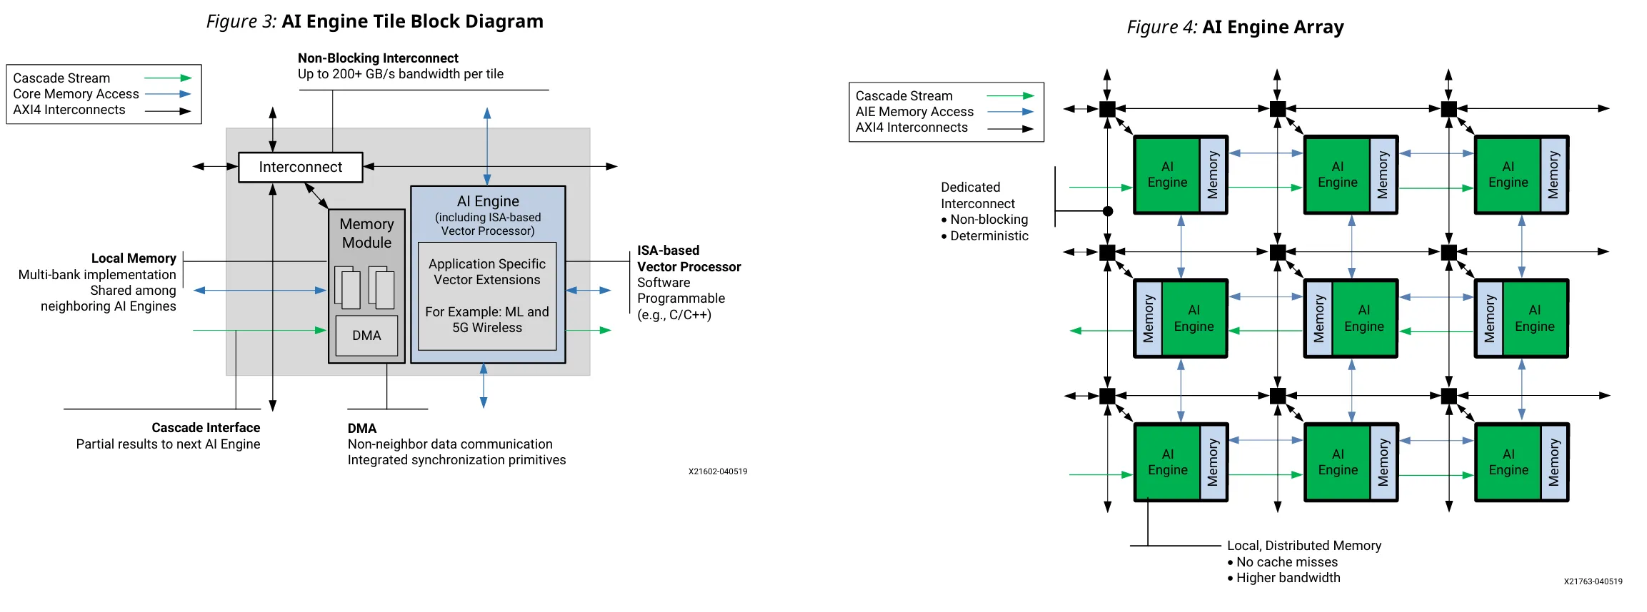
\includegraphics[width=1\linewidth]{archie.png}
    \caption{Cấu trúc chi tiết của AI Engine Tile}
\end{figure}

\begin{itemize}
    \item Tile interconnect: quản lý dữ liệu chạy vào tile qua NoC, PL và được định tuyến tới RAM

    \item AIE Core: có thể lập trình bằng C/C++,… tối ưu cho tính toán song song, có thể cấu hình cho ứng dụng cụ thể, truyền kết quả trung gian tới tile kế tiếp

    \item Memory Module:
    \begin{itemize}
        \item Bao gồm: \textbf{32KB RAM} chia thành 8 bank, DMA, cơ chế đồng bộ giữa các tile.
        \item Khả năng truy cập chéo: mỗi tile có thể truy cập:
        \begin{itemize}
            \item RAM của chính nó.
            \item RAM của tile phía Bắc (North).
            \item RAM của tile phía Nam (South).
            \item RAM của tile phía Đông hoặc Tây (East/West) tùy vào vị trí dòng.
        \end{itemize}
    \end{itemize}

    \item Cascade interface: Các tile được kết nối theo hướng zigzag và hướng lên trên (như minh họa ở Hình 4)
\end{itemize}

\section{Truy cập tài nguyên qua AXI4 MM}

Master AXI4 kết nối vào NoC có thể: đọc ghi RAM của tile, cấu hình bộ DMA, viết lệnh vào thanh ghi control, debug lỗi,…
\begin{figure}[H]
    \centering
    \includegraphics[width=0.75\linewidth]{Pictures/imagecode .png}
    \caption{Địa chỉ giao diện AXI4}
\end{figure}
Cấu trúc địa chỉ: \begin{itemize}
    \item column: tối đa 128 cột
    \item row: tối đa 32 hàng 
    \item tile: offset bên trong tile (để ghi vào thanh ghi, RAM, DMA,…)
\end{itemize}
Ví dụ: Viết từ CPU ARM: ghi 0x42 vào offset 0x100 của tile tại (row=3, col=10): 
\lstinputlisting[style=cstyle, caption={Code}]{codeex.tex}
\section{AXI4-Stream Interconnect\cite{amdAM009}.} 

 Mỗi AIE có 1 AXI4-stream interconnect giúp truyền dữ liệu giữa các tile, cấu hình tĩnh, thông qua giao diện bộ nhớ, có thể lập trình được.\\
 Chức năng: quản lý backpressure (điều tiết dữ liệu khi phía nhận bị nghẽn), đảm bảo băng thông tối đa.\\
 Cấu trúc thành phần:
\begin{itemize}
    \item Port Handlers:
    Điều khiển luồng vào/ra tại mỗi cổng.
    Chọn tuyến đường cho dữ liệu.
    \item FIFOs:
    Hai buffer (bộ đệm) 16 hàng, mỗi hàng rộng 32-bit + 1-bit TLAST.
    Có thể xâu chuỗi (chaining) để tạo độ trễ hoặc buffer dữ liệu.
    \item Arbiters (bộ chọn):
    Sáu bộ chọn lập trình được. 
    Dùng trong chế độ packet switching để phân xử khi nhiều luồng tranh tài nguyên.
    \item Stream Switch Configuration Registers:
    Các thanh ghi cấu hình dùng để thiết lập đường truyền (circuit hoặc packet-switched).
\end{itemize}
\begin{figure}[H]
    \centering
    \includegraphics[width=0.7\linewidth]{Pictures/fig6.png}
    
    \label{fig:enter-label}
\end{figure}
Khối trung tâm chứa các thành phần đã được liệt kê ở trên.\\
Lối vào: 
\begin{itemize}
    \item 4 hướng dữ liệu từ các phía
    \item Form AIE: dữ liệu được tile này sinh ra
    \item From DMA: dữ liệu từ bộ DMA, 
    \item From FIFO: dữ liệu từ bộ FIFO nội bộ
    \item Còn lại là dùng cho debug,...
\end{itemize}
Lối ra: 
\begin{itemize}
    \item 4 hướng dữ liệu đến các phía
    \item To AIE: dữ liệu được gửi đến tile này
    \item To DMA: dữ liệu chuyển tiếp đến nơi khác 
    \item To FIFO: lưu dữ liệu vào FIFO nội bộ
    \item To Register Configuration – cấu hình tuyến hoặc điều khiển chuyển mạch
\end{itemize}

\begin{figure}[H]
    \centering
    \includegraphics[width=0.8\linewidth]{Pictures/table2.png}

    \label{fig:enter-label}
\end{figure}
Ví dụ: nếu tile này muốn gửi dữ liệu sang tile phía đông: dữ liệu từ From AIE đến đầu ra East.

\section{AI Engine Tile Program Memory\cite{amdAM009}}
AIE có bộ nhớ 16KB để lưu câu lệnh VLIW. Có 2 giao diện để quản lý: 
\begin{itemize}
    \item Memory-mapped AXI4 interface: External master có thể đọc/ghi program memory thông qua Memory-mapped AXI4. 
    \item AIE interface:  AIE có giao diện rộng 128bit để nạp lệnh, chỉ có thể đọc mà không thể ghi đến program memory 
\end{itemize}
Để \textbf{truy cập đồng thời cả AIE và AXI4}: Bộ nhớ chia thành nhiều bank, mỗi bên truy cập không trùng nhau. Nếu truye cập trùng, cần có arbitration logic để tránh xung đột, ưu tiên luồng nào trước.

\section{AI Engine Interfaces}
Đọc thêm tại trang 17, tài liệu \cite{amdAM009}.
\begin{table}[h!]
\centering
\caption{Tóm tắt nhanh các giao diện của AI Engine}
\begin{tabular}{l l c}
\hline
\textbf{Giao diện} & \textbf{Mục đích chính} & \textbf{Băng thông / Độ rộng} \\
\hline
Data Memory & Đọc/ghi dữ liệu nội tile & 2×256b load, 1×256b store \\
\hline
Program Memory & Fetch lệnh từ bộ nhớ & 128b \\
\hline
AXI4-Stream (Direct) & Gửi/nhận dữ liệu qua các stream chuẩn & 4×32b (2 in, 2 out) \\
\hline
Cascade Stream & Truyền accumulator giữa tile liền kề & 384b \\
\hline
Debug & Truy cập thanh ghi, hỗ trợ debug & AXI4 \\
\hline
Lock Interface & Đồng bộ hóa hoạt động giữa các tile & -- \\
\hline
Stall Handling & Điều khiển tạm dừng do xung đột hoặc tranh chấp & -- \\
\hline
Event Interface & Giao diện sinh/tạo sự kiện & 16b \\
\hline
Tile Timer & Đếm thời gian nội bộ tile & 64b \\
\hline
\end{tabular}
\end{table}

\section{AIE Architechture}


AIE là bộ xử lý được tối ưu cho:
\begin{itemize}
    \item Single-instruction multiple-data: cho phép thực thi 1 lệnh trên nhiều dư liệu 1 lúc, giúp tăng tốc xử lý các vecto, ví dụ như nhiều phần tử trong ma trận cùng lúc.
    \item Very-long instruction word: cho phép đóng gói nhieeufleenhj vào 1 từ lệnh dài, giúp xử lý song song nhiều lệnh trên 1 chu kì.
    \item Hỗ trợ dấy phẩy động và dấu phẩy tĩnh.
\end{itemize}
Các chức năng của AIE: 
\begin{figure}[H]
    \centering
    \includegraphics[width=0.9\linewidth]{Pictures/fig21.png}
  
    \label{fig:enter-label}
\end{figure}
\begin{itemize}
    \item \textbf{Scalar unit}: Bộ xử lý RISC 32-bit dạng scalar
    \begin{itemize}
        \item Có thanh ghi chung để lưu trữ con trỏ và thanh ghi cấu hình
        \item Hỗ trợ các hàm toán học phi tuyến
        \item Scalar ALU: Bộ xử lý logic số học đơn lẻ, có thể thực hiện nhân 2 số 32 bit scalar
        \item Có khả năng chuyển đổi giữa số nguyên và phẩy động
    \end{itemize}
    \item \textbf{AGU}: 3 bộ sinh địa chỉ  để đọc/ghi dữ liệu từ/to bộ nhớ:
    \begin{itemize}
        \item 2 AGU để load, 1 AGU để lưu
    \end{itemize}
    \begin{itemize}
        \item hỗ trợ nhiều chế độ địa chỉ: địa chỉ không đổi, địa chỉ từ thanh ghi,...
        \item FFT Address Generation: Có phần cứng riêng để tạo địa chỉ đặc biệt phục vụ biến đổi Fourier nhanh (FFT).
    \end{itemize}
    \item  \textbf{Vector fixed-point/integer unit}:
    \begin{itemize}
        \item 32 phép nhân 16-bit có thể được thực hiện mỗi chu kỳ trên một AI Engine tile.
        \item Hỗ trợ phép nhân tích lũy (MAC – Multiply and Accumulate) song song trên nhiều “lane” (đường dữ liệu song song). 
        \item Hỗ trợ dữ liệu real và complex với nhiều độ rộng bit khác nhau (8, 16, 32). (Bảng dưới)
        
        \begin{figure}[H]
        \centering
        \includegraphics[width=0.8\linewidth]{Pictures/table6.png}
        
        \label{fig:enter-label}
    \end{figure}
        \item X, Z là 2 vector đầu vào, X từ thanh ghi 1024 bit và Z từ thanh ghi 256 bit. Do số lương phần tử của Z ít hơn, nên sẽ được sao chép (broadcast) đến nhiều lane để tận dụng tối đa X. Có 128 bộ nhân 8 bit, và kết qua được cộng, lưu vào accumulator.
    \end{itemize}
    \item SPFP (Single-Precision Floating-Point) Vector Unit: Hỗ trợ dấu phẩy động đơn 32bit. Có thể xử lý song song trên nhiều lane, thực hiện 8 đơn vị MAC trên 1 chu kỳ(?)
    \item  \textbf{3 cổng truy cập dữ liệu}: 2 đọc, 1 ghi, có thể hoạt động đồng thời, cần tối ưu layout để tránh xung đột bank, gây stall toàn bộ pipeline.
    \item \textbf{VLIW Function:} Hỗ trợ phát nhiều lệnh tới tất cả function unit, nhiều định dạng khác nhau, độ dài lệnh khác nhau. Tối đa 7 lệnh thực hiện song song trong 1 chu kì.
    
\end{itemize}


    





\newpage
\section{Code Bài tập nhân ma trận AI Engine}
\lstinputlisting[style=cstyle, caption={Code}]{code_mmul.c}
 tài liệu API chính thức của AMD \cite{UG1079}, \cite{MMUL_API}
bài viết giải thích từ Xilinx \cite{XUP_Explained}, và hướng dẫn phòng lab chi tiết \cite{XUP_Lab}.


\chapter{Kết luận và hướng phát triển.}

Qua báo cáo này, em đã hệ thống hóa các kiến thức nền tảng về 5GNR, kiến trúc AI Engine và các thuật toán then chốt trong quá trình mã hóa, giải mã chuỗi PUCCH format 0. Việc triển khai các công thức trên MATLAB đã giúp em hiểu sâu hơn về cách tạo chuỗi giả ngẫu nhiên, tính toán tham số và sinh chuỗi cơ sở, đồng thời kiểm chứng tính chính xác của từng bước thông qua mô phỏng. Tuy nhiên, để mô phỏng sát thực tế hơn, em cần bổ sung các bước truyền chuỗi qua lưới tài nguyên, kênh nhiễu, thực hiện giải mã tín hiệu nhận được nhằm trích xuất thông tin UCI và đánh giá hiệu quả giải điều chế. Đây sẽ là định hướng phát triển tiếp theo của em, đồng thời là tiền đề cho các nghiên cứu chuyên sâu hoặc đề tài tốt nghiệp trong tương lai. Em rất mong nhận được những góp ý quý báu từ cô để hoàn thiện hơn về nội dung và phương pháp nghiên cứu.

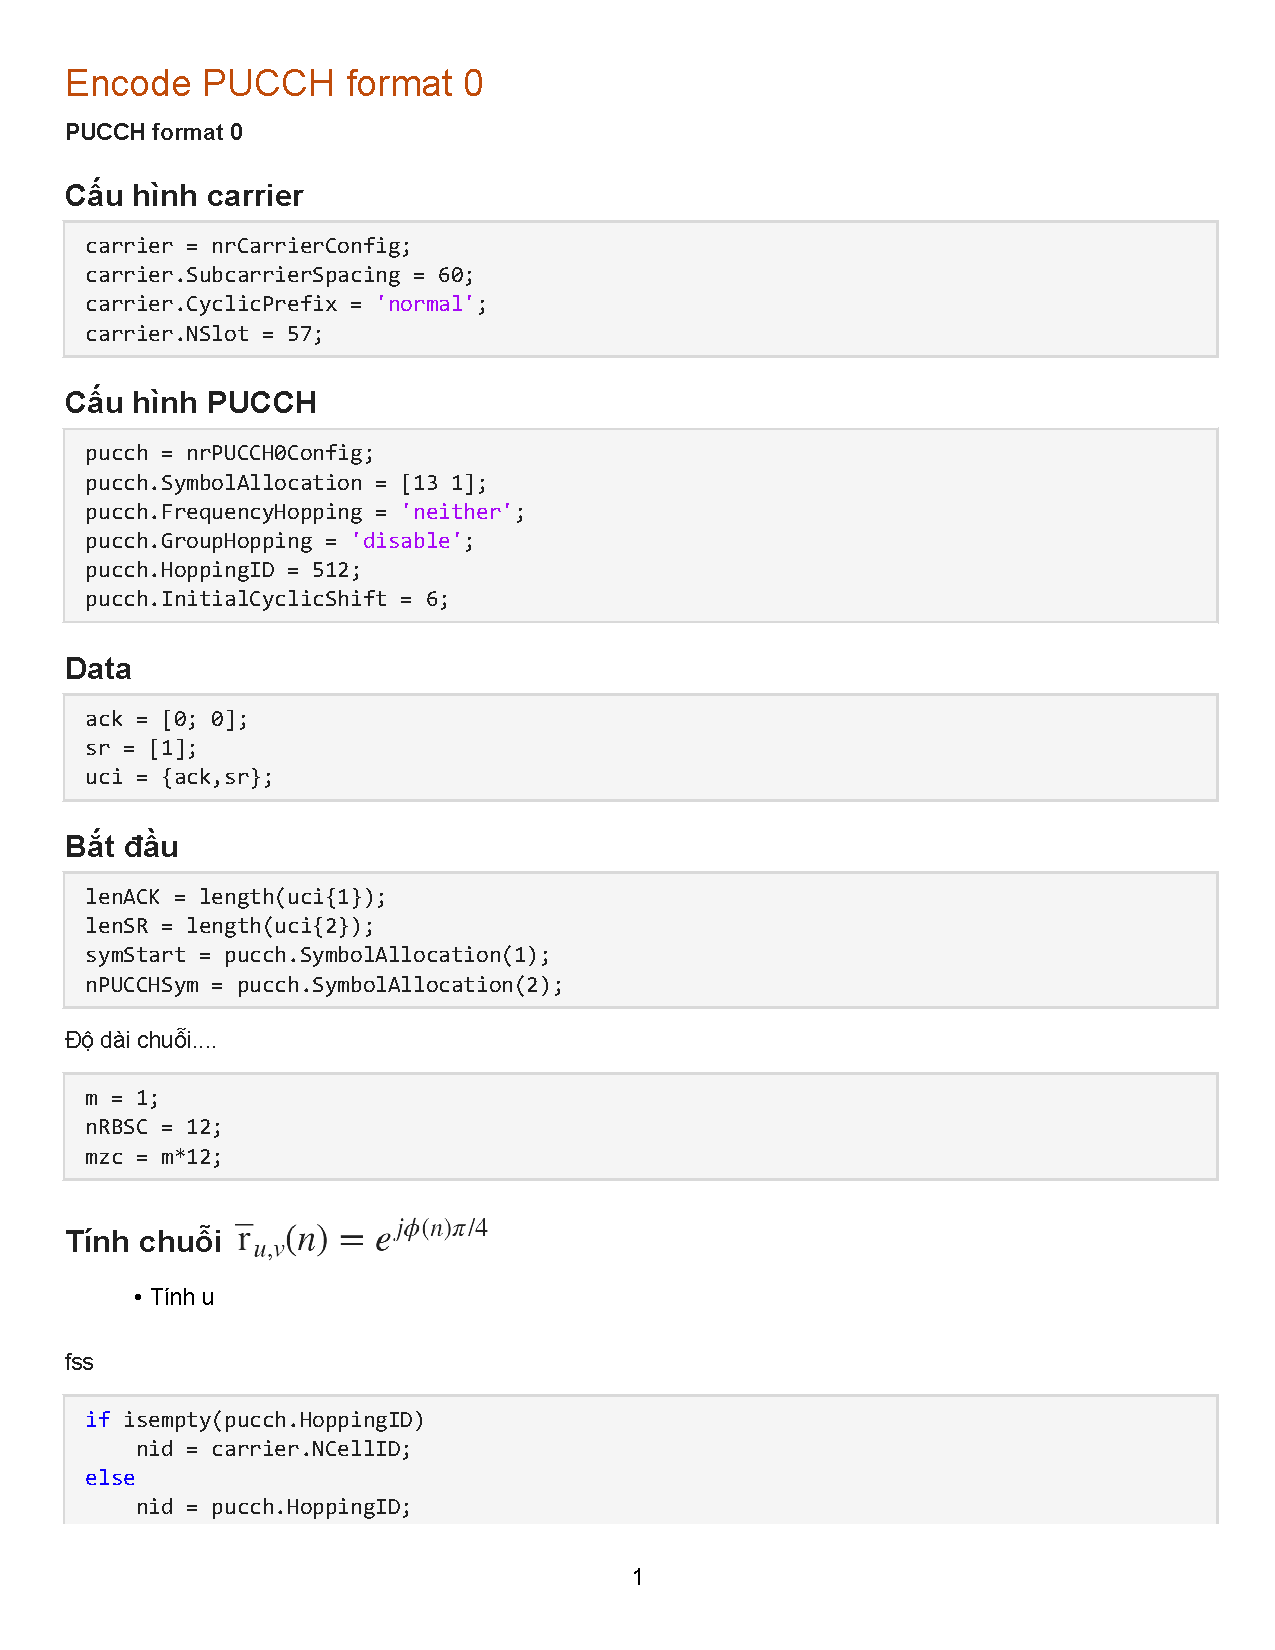
\includepdf[page=-]{EncodeAndDecodePUCCH0.pdf}
\newpage\printbibliography[title={Tài liệu tham khảo}]
\end{document}
